%%%%%%%%%%%%%%%%%%%%%%%%%%%%%%%%%%%%%%%%%%%%%%%%%%%%%%%%%%%%%%%
%
% Welcome to Overleaf --- just edit your LaTeX on the left,
% and we'll compile it for you on the right. If you open the
% 'Share' menu, you can invite other users to edit at the same
% time. See www.overleaf.com/learn for more info. Enjoy!
%
%%%%%%%%%%%%%%%%%%%%%%%%%%%%%%%%%%%%%%%%%%%%%%%%%%%%%%%%%%%%%%%
\documentclass{beamer}

\usetheme{Madrid}
\usecolortheme{lily}
\addtobeamertemplate{footnote}{}{\vspace{2ex}}

\usepackage{amsmath}
\usepackage{amssymb}
\usepackage{color}
\usepackage{listings}
\usepackage{clrscode3e}
\usepackage{multicol}

\definecolor{codegreen}{HTML}{237e02}
\definecolor{codegray}{rgb}{0.5,0.5,0.5}
\definecolor{codepurple}{HTML}{8F4673}
\definecolor{codebrown}{HTML}{ce9178}
\definecolor{codecyan}{HTML}{098658}
\lstdefinestyle{pythonstyle}{
    commentstyle=\color{codegreen},
    keywordstyle=\color{codepurple},
    numberstyle=\tiny\color{codegray},
    stringstyle=\color{codebrown},
    basicstyle=\ttfamily\small,
    breakatwhitespace=false,         
    breaklines=true,                 
    captionpos=b,                    
    keepspaces=true,                 
    numbersep=5pt,                  
    showspaces=false,                
    showstringspaces=false,
    showtabs=false,
    tabsize=2
}
\def\And{\text{ AND }}
\def\Or{\text{ OR }}
\def\Xor{\text{ XOR }}
\def\Implies{\text{ IMPLIES }}
\def\Iff{\text{ IFF }}
\def\Not{\text{NOT}}
\def\R{\mathbb{R}}
\def\N{\mathbb{N}}
\lstset{style=pythonstyle}

\setlength{\parskip}{1em}

%Information to be included in the title page:
\title{Format for Efficient Storage of Homology Relations}
\subtitle{Week 5 Report: Python Parser Test and Preliminary Benchmark for VTD-XML}
\author{Kevin Gao}
\institute{University of Toronto}

\begin{document}

\frame{\titlepage}

\AtBeginSection[]
{
    \begin{frame}
    \frametitle{Outlines}
    \tableofcontents[currentsection]
    \end{frame}
}

\section{Correctness of ETE3-based APIs}

\begin{frame}{ETE-based API}
    As mentioned in last week's report, ETE3 is a Python-based, open-sourced bioinformatics package. The underlying implementation uses \texttt{lxml}, a DOM-based parser. Recall that a DOM parser parses an XML file into a tree structure in the memory.

    Last week, I presented a few examples of the simple APIs I have developed using the parser that comes with ETE3 on some small trees. This week, we expanded the test set into larger and more complex trees.
\end{frame}

\begin{frame}{ETE-based API}
    After annotating the XML file with speciation/duplication events, we tested the APIs on two large datasets: the gene trees for BRCA2 and RNU6-92P.

    First, to test if our annotation algorithm is correct, we can print out the number of duplication and speciation nodes.

    \begin{table}[htbp]
        \centering\begin{tabular}{c|c|c|c|c}
            Dataset & \shortstack{Reported \\ speciations} & \shortstack{Reported \\ duplications} & \shortstack{Actual \\ speciations} & \shortstack{Actual \\ duplications} \\
            \hline
            BRCA2 & 168 & 7 & 168 & 3 \\
            \hline
            RNU6-92P & 289 & 79 & 289 & 51
        \end{tabular}
    \end{table}
    For BRCA2, there are 3 ambiguous nodes and 1 gene split node. For RNU6-92P, there are 28 ambiguous nodes. If we add those to the actual duplications count, we get the same number as the reported number.
\end{frame}

\begin{frame}{ETE-based API}
    A pairwise test of homologous genes shows that homology inference can be done correctly, except for gene split and ambiguous nodes. Ambiguous relations can be determined by checking the confidence score (which is also included in the annotated phyloXML file). Gene split would likely require additional annotations (or a richer format like recPhyloXML).
\end{frame}

\begin{frame}{Benchmark Results}
    We benchmarked the APIs based on the following metrics.

    Parsing time (1000 executions): 35.605456083s \\
    Parsing speed: 30.64 MB/s \\
    Homology inference time (10000 execution): 48.6419415s \\
    Homology inference speed: 205.58 ops/s

    Avg parsing speed: 30-36 MB/s \\
    Avg homology inference speed: 150-200 ops/s

    The parsing speed is calculated as follows
    $$
    \frac{\text{file size (in bytes)} \times \text{repetitions}}{\text{time elapsed} \times 2^{20}}
    $$
\end{frame}

\section{VTD index for XML}
\begin{frame}{VTD-XML Parser}
    VTD stands for virtual token descriptor. A VTD record is a 64-bit binary value organized as follows.

    \begin{figure}[htbp]
        \centering
        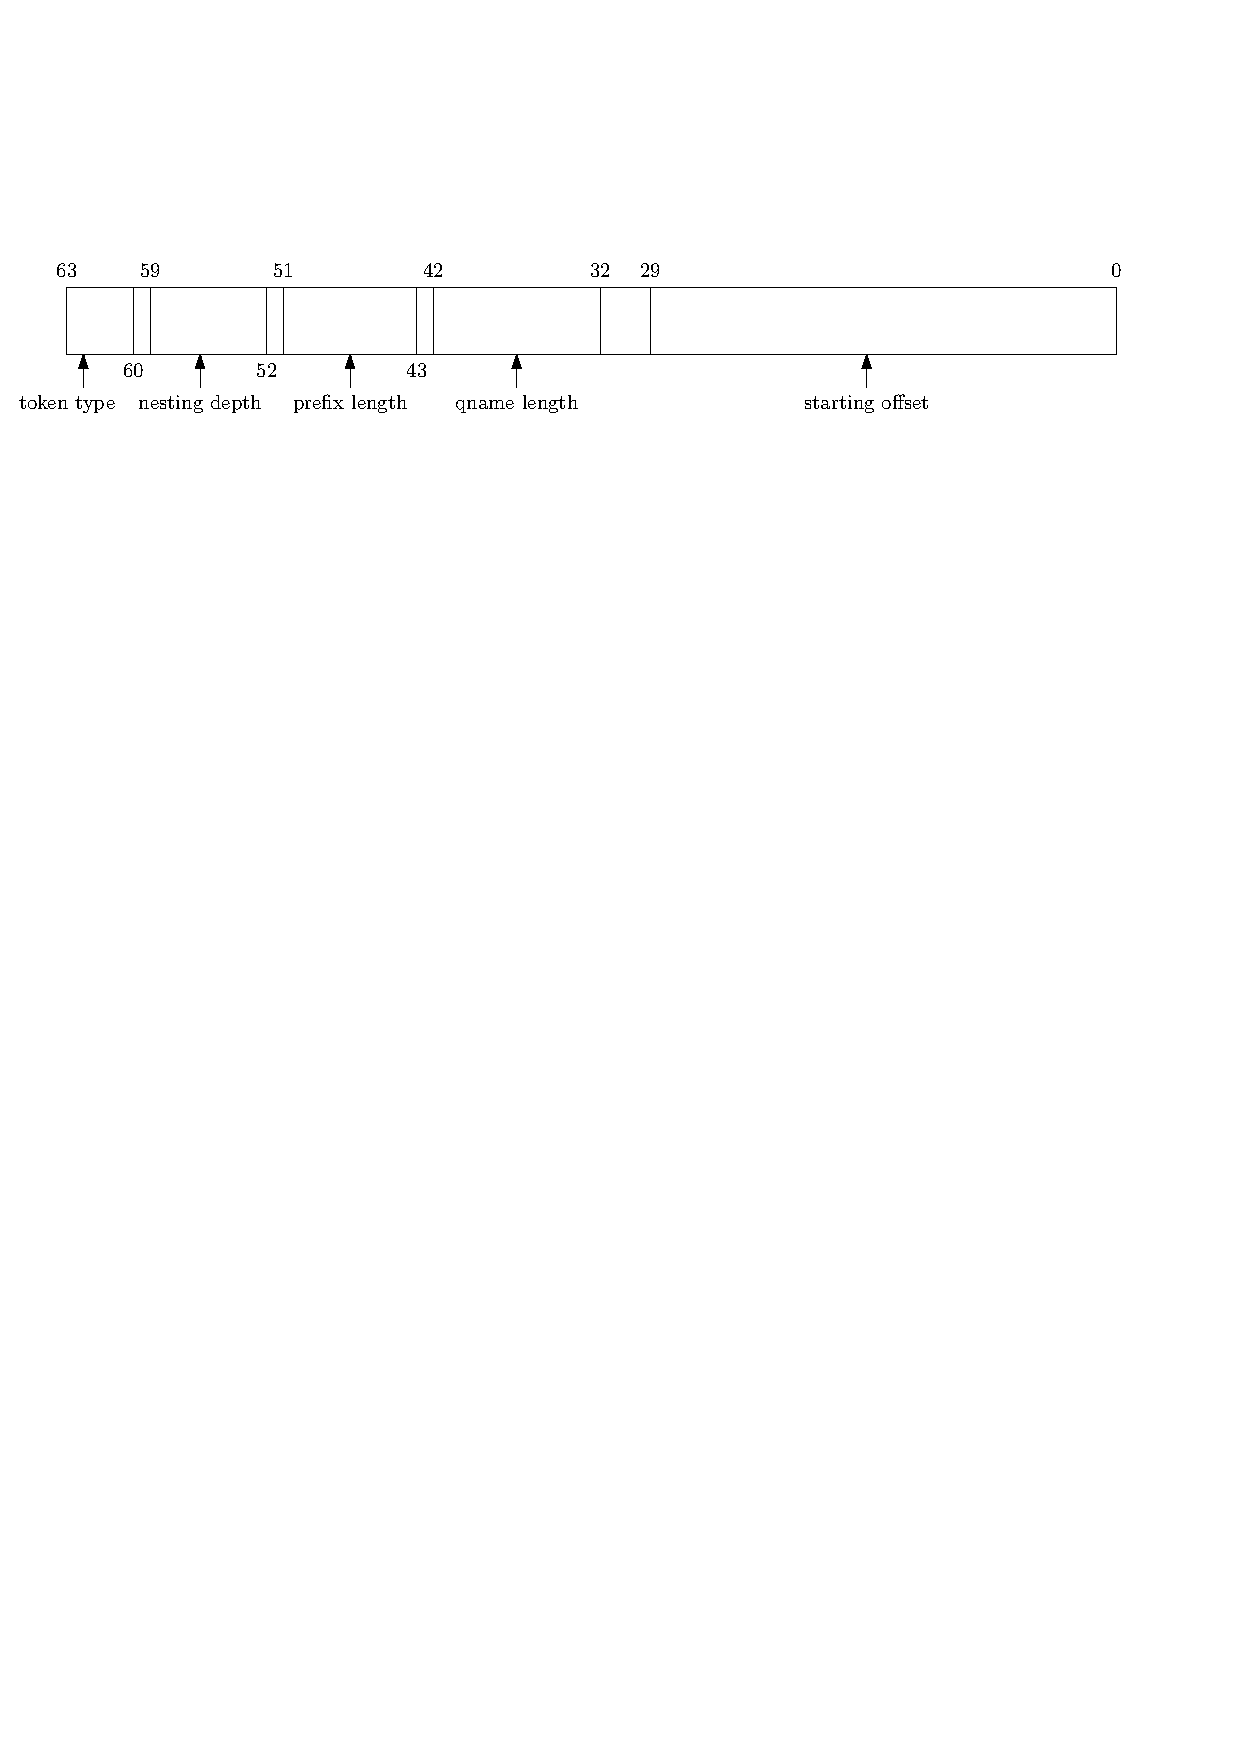
\includegraphics[width=\linewidth]{res/vtd-record-schematic.pdf}
    \end{figure}

    In addition to VTD records, we have an LC (location) cache records for each token. Based on the configuration, there can be 3 or 5 levels of LC.

    \begin{figure}[htbp]
        \centering
        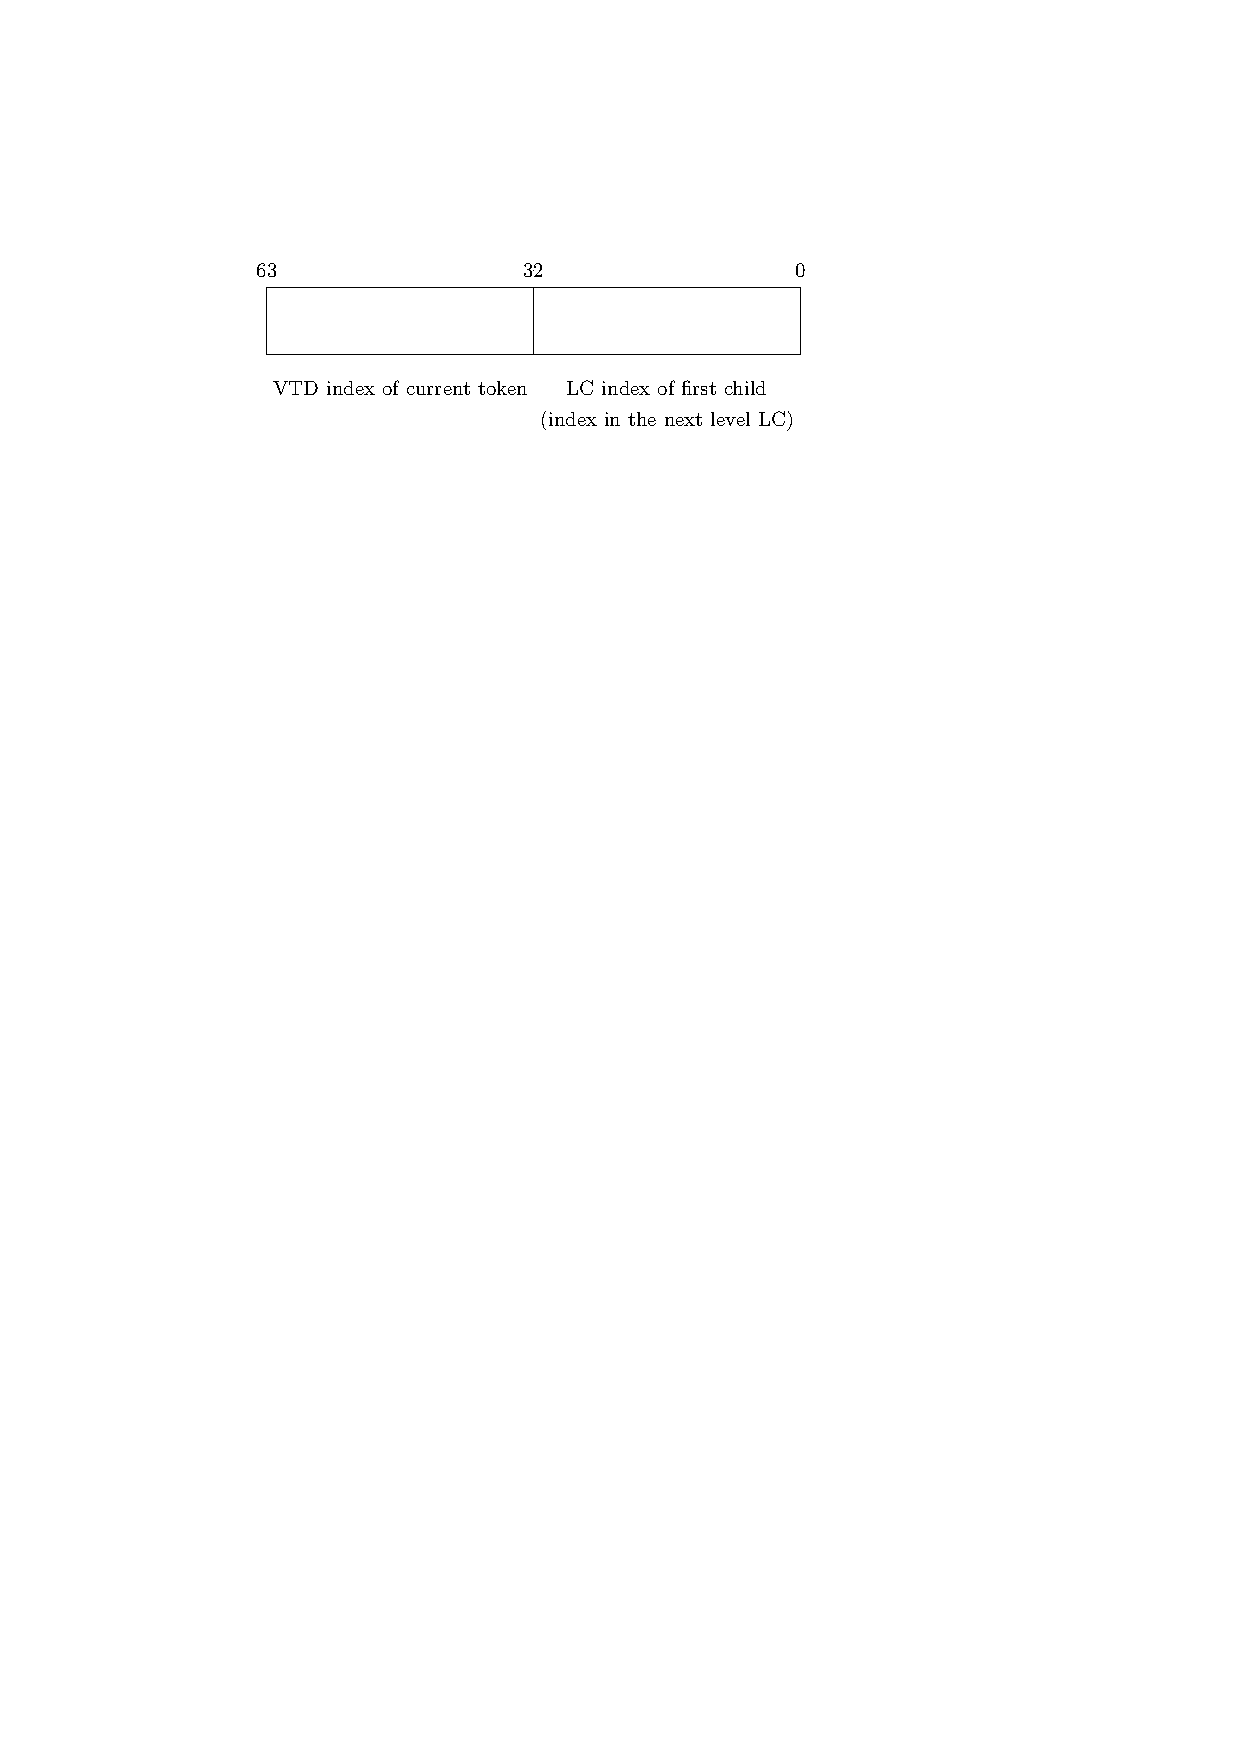
\includegraphics[width=0.5\linewidth]{res/lc-record-schematic.pdf}
    \end{figure}
\end{frame}

\begin{frame}{VTD As Index}
    VTD records can be naturally used as an index for XML files as it allows for efficient random access while keeping a low memory footprint.

    In addition, we can integrate the binary VTD records and LC records into XML files, creating a binary format known as VTD-XML.

    However, one issue with indexing with VTD is that the depth level for LC (location cache) is a constant (either 3 or 5) and might not be sufficient for trees with a large height. Additionally, LC keeps track of descendant relations, but for our purposes, we are more interested in \textbf{ancestry relations}.
\end{frame}

\begin{frame}{Parsing Speed For VTD}
    The VTD parser is ported to C++ and preliminary benchmarking on parsing speed shows promising results compared to our naive parser. The parsing speed can be as fast as 385 MB/s. 
    
    The fast speed is partly due to C++ being a compiled language but the efficiency of VTD parsers could also contribute to the speed improvement.

    The original parser is quite complicated as it needs to consider support for different XML encodings and XPath queries. We will eventually remove these components as appropriate to have a more lightweighted and easy-to-maintain parser.
\end{frame}

\section{References}

\begin{frame}
    \scriptsize

    Zhang, J., Lovette, K.: XimpleWare W3C Position Paper. In: W3C Workshop on Binary Interchange of XML Information Item Sets (2003)
\end{frame}

\end{document}